\section{Sprint 9: Comentarios, notificaciones y grupos}



\subsection{Descripción}

En el sprint anterior se desarrolló la funcionalidad necesaria para poder compartir análisis y enviar notificaciones de este evento, al usuario objetivo de la compartición. Esta interacción es muy útil pero el objetivo del equipo es brindar funcionalidades que permita a los usuarios interactuar intercambiando mensajes de forma instantánea. Para lograr esto, el equipo desarrolla la funcionalidad de comentarios, permitiendo a un usuario realizar una nota sobre un análisis y brindarle la posibilidad, al usuario dueño del análisis, ver estos comentarios y agregar nuevos. 

De esta forma cuando un paciente comparte un análisis con un médico, éste último podrá ver los resultados de los estudios e indicar mediante un comentario, ciertas recomendaciones como que es necesario que se acerque al consultorio para poder darle una devolución y diagnóstico o si el diagnóstico es simple poder indicar la situación en el comentario del análisis o cargar el diagnóstico como una imagen al análisis. Este tipo de interacción entre usuarios genera un nuevo tipo de eventos en el sistema que deben ser dados a conocer al usuario que corresponda en el momento que ocurren, para esto se definen notificaciones específicas para comentarios.

Por otro lado el equipo considera que el sistema tiene una gran cantidad de usuarios que por algún motivo no pueden usar el sistema, sin embargo esto no les debería impedir explotar las facilidades que el mismo puede brindarles. Los casos son muy variados, desde personas mayores que no se encuentran familiarizados con éste tipo de tecnologías a personas menores que no poseen edad suficiente como para manejarlas. 

Para salvar esta situación se ha definido grupos con una membresía representativa de su objetivo y un tipo de permiso, los grupos estarán conformados por usuarios los cuales también tendrán un tipo de membresía que lo representa como por ejemplo ``Padre'' en un grupo familiar, además tendrán un tipo de permiso y se deberá indicar si es o no administrador del grupo. Suponiendo el caso del grupo familiar, esta funcionalidad permitiría a un usuario administrador con membresía ``padre'' agregar un hijo al grupo y, si este no tiene edad suficiente para manejar el sistema, el padre puede tener los permisos adecuados para gestionar sus análisis y permitir una carga temprana de datos históricos del usuario. Cómo esta nueva funcionalidad incorpora nuevos eventos, es pertinente definir las notificaciones adecuadas para comunicarlos.

Luego de una reunión con interesados en el sistema el equipo releva la necesidad de definir un rango de unidades válidos para las medidas ingresadas al sistema, para esto se desarrollan validaciones de unidades que alertan al usuario cuando se exceden los valores considerados normales.

Para identificar al usuario, por ejemplo cuando se busca para compartir un análisis, el equipo decide desarrollar lo necesario para obtener el gravatar público definido por el usuario.

Este sprint le permite al usuario:
	\begin{itemize}
		\item Comentar análisis compartidos por un usuario.
		\item Recibir notificaciones por comentarios.
		\item Crear grupos.
		\item Agregar usuarios a grupos.
		\item Definir tipos de membresías para los usuarios agregados a un grupo.
		\item Definir tipos de permiso para los usuarios agregados a un grupo.
		\item Compartir análisis a un grupo del que forma parte el usuario.
		\item Recibir notificación por compartición de un análisis de un usuario que forma parte del mismo grupo.
		\item Recibir notificación al ser agregado a un grupo.
	\end{itemize}

\subsection{User Stories relacionados}
La \textbf{Tabla \ref{US-Sprint9}} indicará las características de cada user story para guiarnos en el desarrollo del sprint.

\begin{table}[h]
    \centering
	\begin{tabular}{|l|p{9cm}|}
	\hline
        \multicolumn{1}{|c|}{\textbf{ID}} &
        \multicolumn{1}{|c|}{\textbf{Enunciado de la historia}} \\          
    \hline
        US-\ref{evitarPerdidas} &
        Como paciente, quiero  añadir al sistema mis estudios realizados para evitar posibles pérdidas.\\
    \hline
       	US-\ref{agregarGrupoFamiliar} &
       	Como paciente, quiero agregar personas a mi grupo familiar, para llevar el seguimiento de los mismos. \\
    \hline
       	US-\ref{modificarPermisos} &
       	Como paciente, quiero modificar los permisos de visualización de mis datos con respecto a cada uno de los integrantes del grupo familiar, para tener un control total sobre mi privacidad. \\
    \hline 
        US-\ref{comunicarResultado} &
        Como paciente quiero que no sea necesario ir al hospital para que un médico me comunique los resultados del análisis.\\
    \hline
       	US-\ref{infoHijo} &
       	Como mujer embarazada, quiero llevar la información de mi hijo, para transmitírsela cuando nazca. \\
    \hline
    	US-\ref{accesoCualquierLugar} &
    	Como paciente, quiero acceder a mis documentos desde cualquier lugar, para hacer uso de ellos cuando los necesite. \\
    \hline
        US-\ref{mostrarComentario} &
        Como paciente quiero ver en un único lugar los comentarios realizados por los médicos autorizados para una lectura rápida.\\
    \hline     
        US-\ref{validarUsuario} &
        Como paciente, quiero contar con un acceso único y privado a mi información, para que no sea accedida por usuarios sin permisos.\\
    \hline
    \end{tabular}
    \caption{Listado de \textit{User Stories} relacionados.}
    \label{US-Sprint9}
\end{table}
\subsection{Planificación}
\subsubsection{Período de realización}
\begin{itemize}
	\item \textbf{Inicio}: 01 de Noviembre de 2015.
	\item \textbf{Fin}: 20 de Noviembre de 2015.
\end{itemize}


\subsubsection{Sprint backlog}

{\scriptsize
	\begin{center} %sidewaystable
		\centering
		%\begin{adjustbox}{max width=\textheight}
		\resizebox{\textwidth}{!}{
			\begin{tabular}{|l|l|l|p{6cm}|l|l|}
				\hline
				\textbf{Área a cargo} &
				\textbf{Responsable} &  
				\textbf{Revisor} &       
				\textbf{Tarea} &
				\textbf{US} &
				\textbf{tiempo dedicado}\\ 
				\hline
				Back-end& Michael Manganiello & Franco Canizo & Funcionalidad de comentado de análisis & US-\ref{comunicarResultado} \& US-\ref{mostrarComentario} & 20hs \\ 
				\hline
				Back-end& Michael Manganiello & Franco Canizo & Funcionalidad grupos de usuario & US-\ref{comunicarResultado} \& US-\ref{validarUsuario} & 36hs \\ 
				\hline
				Back-end& Michael Manganiello & Franco Canizo & Incorporación de permisos a grupos de usuarios & US-\ref{comunicarResultado} \& US-\ref{validarUsuario} & 18hs \\ 
				\hline
				Back-end& Michael Manganiello & Franco Canizo & Implementación validaciones para unidades de medición & US-\ref{infoPerfil} \& US-\ref{infoSalud} & 6hs \\
				\hline
				Back-end& Michael Manganiello & Franco Canizo & Incorporació de la imagen Gravatar de un usuario & US-\ref{infoPerfil} \& US-\ref{infoSalud} & 14hs\\ 
				\hline
				Back-end& Michael Manganiello & Franco Canizo & Desarrollo de nuevos tipos de notificación & US-\ref{infoPerfil} \& US-\ref{infoSalud} & 10hs\\ 
				\hline
				Back-end& Michael Manganiello & Franco Canizo & Compartición de análisis a grupo & US-\ref{comunicarResultado} \& US-\ref{infoHijo} \& US-\ref{mostrarComentario} & 10hs\\ 
				\hline
				Back-end& Franco Canizo & Michael Manganiello & Implementación del adaptador para la conexión con Drive & US-\ref{accesoCualquierLugar} \& US-\ref{evitarPerdidas} & 24hs\\ 
				\hline
				Documentación & Franco Canizo & Michael Manganiello & Documentación de los sprints 7, 8 y 9  & - & 48hs\\ 
				\hline
			\end{tabular}
		}
		%\end{adjustbox}
	\end{center}
}

\subsection{Modelo funcional} 
Se describirán las funciones usando como marco de apoyo el sprint Backlog, además se armará el diagrama de casos de uso del presente Sprint \textbf{[Figura \ref{dcu-sprint-9}]} que irá creciendo  medida se vaya avanzando en el proyecto.

    \begin{figure}[h]
        \centering
        \includegraphics[width=0.5\textwidth]{img/dcu_sprint9}
        \caption{Funcionalidades comentarios, notificaciones y grupos.}
		\label{dcu-sprint-9}
    \end{figure}
    
\subsection{Modelo de datos}
El Diagrama propio de este sprint se puede ver en la \textbf{Figura \ref{9-clases_comentario_grupos}}, allí se indican exactamente las clases que se usarán en este sprint y que serán detalladas con detenimiento en el presente documento. Se recuerda que se ha realizado un Diagrama de clases específico para este sprint y puede variar en futuras iteraciones.

    \begin{figure}[h]
        \centering
        \includegraphics[width=0.5\textwidth]{img/dc_sprint9}
        \caption{Clases para comentarios, notificaciones y grupos.}
		\label{9-clases_comentario_grupos}
    \end{figure}

\begin{comment}
\subsection {Salidas del Sistema - Incrementos}
\textbf{Esto es un ejemplo. Debe listarse las pantallas y explicar que hacen}
\begin{enumerate}
   \item \textbf{Presentación de las últimas mediciones}  \textbf{[Figura  \ref{perfil_medicion}]} con posibilidad de edición de cada una de las mediciones. Los datos posible  a presentar son altura, peso, grasa corporal y glucosa. 
  
    La interfaz mostrará el valor de la medición, la fecha y hora en que fue realizada y la fuente que se utilizó para dicha medición.

\end{enumerate}
\end{comment}

\subsubsection{Modelos para comentarios, notificaciones y grupos}

Para el manejo de comentarios se definen los modelos \textbf{AnalysisComment} que modela el comentario de un perfil de usuario sobre un análisis específico. Tiene como atributos la fecha y hora en que se realizó el comentario, el comentario específico y las relaciones con el análisis que se comenta y el perfil que comenta el análisis. En el siguiente diagrama [\ref{9-comentario_análisis}] se hace foco sobre el modelo correspondiente.

	\begin{figure}[h]
        \centering
        \includegraphics[width=0.5\textwidth]{img/dc_coment}
        \caption{Clases comentarios.}
		\label{9-comentario_análisis}
    \end{figure}

Los comentarios, al igual que los archivos y medidos están relacionados con un análisis, por lo tanto definimos nuevos tipos de permisos en el modelo \textbf{PermissionType} a través de los atributos can\_view\_comments can\_edit\_comments.

Para la definición de grupos se definen los modelos \textbf{Group} que representa un grupo de usuarios (concretamente, de perfiles de usuario), con nombre y descripción del grupo, \textbf{GroupMembershipType} que lista los tipos de miembros en un grupo. En caso de un grupo familiar, los diferentes tipos de membresías pueden ser "Padre", "Hijo", "Médico de cabecera", entre otros. Por último el modelo \textbf{GroupMembership} que indica el perfil de usuario, el grupo al que pertenece, el tipo de miembro y el tipo de permiso que tiene el usuario sobre todos los análisis de los miembros del grupo, en resumen, la forma en que ese Usuario se desempeñará en el grupo según el administrador. 

El modelo es el siguiente [\textbf{Figura \ref{9-grupo}}]

	\begin{figure}[h]
        \centering
        \includegraphics[width=0.9\textwidth]{img/dc_grupos}
        \caption{Clases grupos.}
		\label{9-grupo}
    \end{figure}

Para la gestión de notificaciones se definen 3 modelos: \textbf{NotificationNewAnalysisFromGroup} que notifica al usuario cuando un nuevo análisis ha sido compartido por algún miembro en uno de sus grupos, \textbf{NotificationNewGroupMembership} que notifica al usuario cuando ha sido agregado como miembro a un nuevo grupo. y por último \textbf{NotificationNewAnalysisComment}  que notifica al dueño de un análisis, cuando alguien realiza un comentario en el mismo. La siguiente figura [\ref{9-notificaciones}] muestra como queda la lógica de notificaciones. 

	\begin{figure}[h]
        \centering
        \includegraphics[width=0.9\textwidth]{img/dc_notification}
        \caption{Clases notificaciones.}
		\label{9-notificaciones}
    \end{figure}

Para la validación de unidades se desarrollo el modelo \textbf{TypeUnitValidation} que indica, para cada tipo de medición, sus unidades de medición y los valores mínimos y máximos propuestos para cada una de las mismas. El modelo es el siguiente [\ref{9-validaciones}]

	\begin{figure}[h]
        \centering
        \includegraphics[width=0.5\textwidth]{img/dc_validaciones}
        \caption{Clases validaciones.}
		\label{9-validaciones}
    \end{figure}

Se define la funcionalidad para la compartición de análisis a un grupo determinado. Para esto se define el modelo \textbf{GroupPermission} que describe el permiso de un grupo a un análisis específico.

\subsubsection{Definición de recursos}

Para comentarios se definen los siguientes recursos:
\begin{itemize}
	\item \textbf{AnalysisAnalysisCommentList}. Mediante el método GET, ofrece el servicio de devolver todos los comentarios asociados al análisis, ordenados por fecha  siempre que el usuario que esté consultandolos esté autenticado y tenga permisos para con el análisis específico. Mediante el método POST ofrece el servicio de permitir crear un nuevo comentario para el análisis siempre que tenga permisos para con el análisis específico.
	\item \textbf{AnalysisCommentView}. Mediante el método GET ofrece el servicio de devolver la información del comentario especificado. Mediante PUT (autenticado como el creador del comentario), permite modificar solamente el contenido del comentario.
\end{itemize}

Para grupos se definen los siguientes recursos:
\begin{itemize}
	\item \textbf{GroupList} mediante el servicio POST permite crear una nueva instancia de grupo, y una membresía de grupo asociada al perfil del usuario autenticado. Retorna la instancia de grupo. Requiere los datos de la nueva membresía, para crearla y asociarla al usuario autenticado, como nuevo administrador del grupo.
	
	\item \textbf{GroupView} mediante el servicio GET retorna una instancia específica de grupo. Requiere autenticación, y ser un miembro del grupo solicitado. PUT actualiza una instancia específica de grupo, y la retorna. Requiere autenticación, y ser un administrador del grupo. DELETE elimina una instancia específica de grupo, junto a todas sus membresías asociadas. Requiere autenticación, y ser un administrador del grupo.
	
	\item \textbf{GroupGroupMembershipList}. El servicio GET retorna todas las instancias existentes de membresías de grupo, asociadas a un grupo específico. Requiere autenticación, y ser un miembro del grupo. POST crea una nueva instancia de membresía de grupo, asociada al perfil del usuario indicado y al grupo especificado, y la retorna. Requiere autenticación, y ser un administrador del grupo.
	
	\item \textbf{GroupMembershipTypeList}. GET retorna todas las instancias existentes de tipo de membresía de grupo. POST crea una nueva instancia de tipo de membresía de grupo, y la retorna.
	
	\item \textbf{GroupMembershipTypeView}. GET retorna una instancia específica de tipo de membresía de grupo. PUT actualiza una instancia específica de tipo de membresía de grupo, y la retorna.
	
	\item \textbf{GroupMembershipView}. GET retorna una instancia específica de membresía de grupo. PUT actualiza una instancia específica de membresía de grupo, y la retorna. Sólo permite modificar si la membresía es de administrador, su tipo de membresía y el tipo de permiso asociado. Requiere autenticación, y ser un administrador del grupo. DELETE elimina una instancia específica de membresía de grupo. Requiere autenticación, y ser un administrador del grupo, o el dueño de la membresía especificada.
	
	\item \textbf{MyGroupList} el servicio GET retorna todas las instancias existentes de grupos, en las que el usuario autenticado tiene membresía.
	
	\item \textbf{MyGroupMembershipList}  mediante el servicio GET, retorna todas las membresías de grupo asociadas al usuario autenticado. Si el parámetro query opcional de tipo entero: group está seteado, se filtran las membresías para solo obtener las asociadas al grupo.
	
\end{itemize}

Recursos para validaciones:

\begin{itemize}
	\item \textbf{TypeUnitValidationList}. Mediante GET, retorna todas las validaciones de unidad de medición, asociadas al tipo de medición especificado. Mediante POST, permite crear una nueva validación de unidad de medición para el tipo de medición indicado.
	\item \textbf{TypeUnitValidationView}. Mediante GET, retorna la instancia específica de validación de unidad de medición. Mediante PUT, actualiza los atributos propios de la instancia especificada de validación de unidad de medición. Mediante DELETE, elimina la instancia indicada.
	
	
\end{itemize}

Recursos para obtener el gravatar a partir de una url:

\begin{itemize}
	\item \textbf{UserGravatarView} mediante GET, retorna la dirección URL de la imagen Gravatar del usuario especificado.
    \item \textbf{MyGravatarView}: Mediante GET, retorna la dirección URL de la imagen Gravatar del usuario autenticado.
\end{itemize}

Utilizando además el parámetro default podemos obtener la imagen por defecto, en caso de no existir un gravatar asociado a la dirección de correo electrónico del usuario. El parámetro size nos permite determinar el tamaño en píxeles de la imagen solicitada. Debido a que son imágenes cuadradas, sólo se requiere un número, entre 1 y 2048. Por defecto, la imagen es de 80px.

Recursos para compartición de un archivo a un grupo:
    \textbf{AnalysisGroupPermissionList} mediante GET, retorna todos los permisos de grupo del análisis. Mediante POST, estando autenticado y siendo el dueño del análisis especificado, crea un nuevo permiso de grupo para el mismo.
    \textbf{GroupPermissionView} mediante GET, retorna la instancia específica de permiso de grupo. Mediante DELETE, estando autenticado y siendo el dueño del análisis asociado al permiso especificado, elimina el mismo.

\subsubsection{Identificadores}
    
Identificadores para hacer uso de los recursos correspondientes a comentarios:

Identificadores para los recursos de grupos:
\begin{itemize}
	\item \textbf{/groups} para el recurso GroupList.
	\item \textbf{/groups/<group\_id>} para el recurso GroupView.
	\item \textbf{/groups/<group\_id>/members} recurso GroupGroupMembershipList.
	\item \textbf{/group\_membership\_types} recurso GroupMembershipTypeList.
	\item \textbf{/group\_membership\_types/<group\_membership\_type\_id>} recurso GroupMembershipTypeView.
	\item \textbf{/group\_memberships/<group\_membership\_id>} recurso GroupMembershipView.
	\item \textbf{/my/groups} recurso MyGroupList.
	\item \textbf{/my/group\_memberships} recurso MyGroupMembershipList.
\end{itemize}

Identificadores para validaciones:

\begin{itemize}
	\item \textbf{/measurement\_types/<int:measurement\_type\_id>/unit\_validations} recurso TypeUnitValidationList
	\item \textbf{/type\_unit\_validations/<int:type\_unit\_validation\_id>} recurso TypeUnitValidationView 
\end{itemize}

Identificadores para gestión de gravatar:

\begin{itemize}
	\item \textbf{/users/<int:user\_id>/gravatar} recurso UserGravatarView.
	\item \textbf{/my/gravatar} recurso MyGravatarView.
\end{itemize}


\subsection{Salidas del sistema}
Luego de finalizado este Sprint se obtendrán 4 pantallas que se detallarán a continuación:

	\begin{itemize}
		\item \textbf{Comentar análisis compartidos por un usuario:} Se le perite l usuario realizar comentario sobre un análisis en particular. \textbf{[Figura \ref{realizar_comentario}]}
		\item \textbf{Recibir notificaciones por comentarios:} Desde la barra horizontal se le brinda al usuario iconos que representan las notifcaciones correspondiente a comentarios. En este ícono se muestra cantidad de mensajes no leídos y al presionarlo se indica quien ha sido el emisor de dicho mensaje. \textbf{[Figura \ref{notificacion_mensaje}]}
		\item \textbf{Crear grupos: } Se muestra una vista de los grupos creados por el usuario. \textbf{[Figura  \ref{grupos}]}
		\item \textbf{Crear grupo: } Se genera el formulario para la creación de grupos 
		\item \textbf{Agregar usuarios a grupos.} Se genera un dormulario para añadir un nuevo usaurio al grupo \textbf{[Figura \ref{nuevo_usuario_grupo}]}
		\item \textbf{Compartir análisis a un grupo del que forma parte el usuario.} Se genera el formulario para compartir un análisis con un grupo, \textbf{[Figura \ref{compartir_analisis_grupo}]}
	\end{itemize}
	
	
	    \begin{figure}[h]
	    	\centering
	    	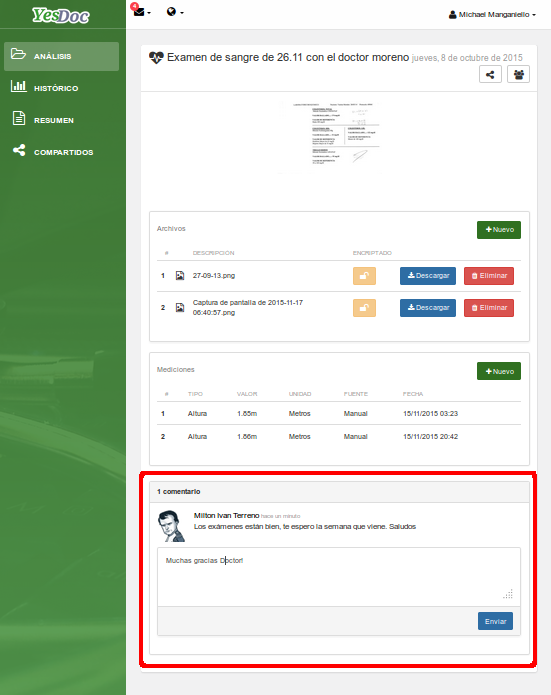
\includegraphics[width=0.5\textwidth]{img/realizar_comentario}
	    	\caption{Sección de comentarios en un análisis}
	    	\label{realizar_comentario}
	    \end{figure}


	    \begin{figure}[h]
	    	\centering
	    	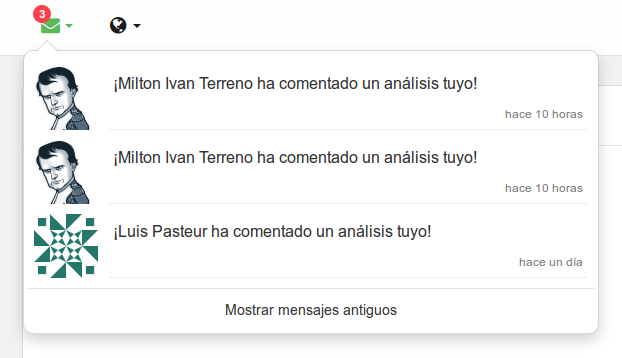
\includegraphics[width=0.5\textwidth]{img/notificacion_mensaje}
	    	\caption{Notificaciones de los mensajes}
	    	\label{notificacion_mensaje}
	    \end{figure}	
	    \begin{figure}[h]
	    	\centering
	    	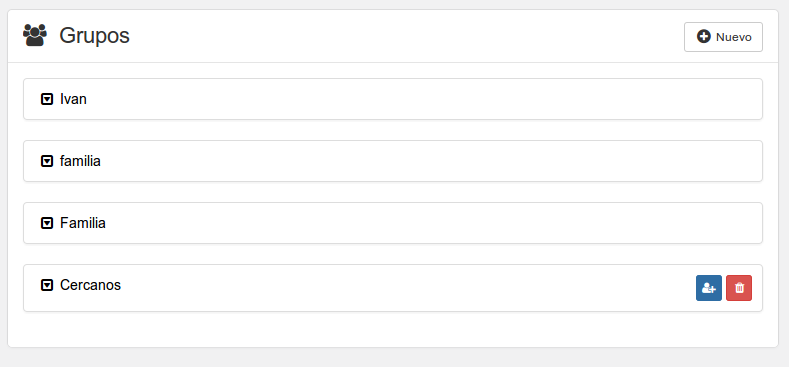
\includegraphics[width=0.5\textwidth]{img/grupos}
	    	\caption{Lista de grupos}
	    	\label{grupos}
	    \end{figure}	    

	    \begin{figure}[h]
	    	\centering
	    	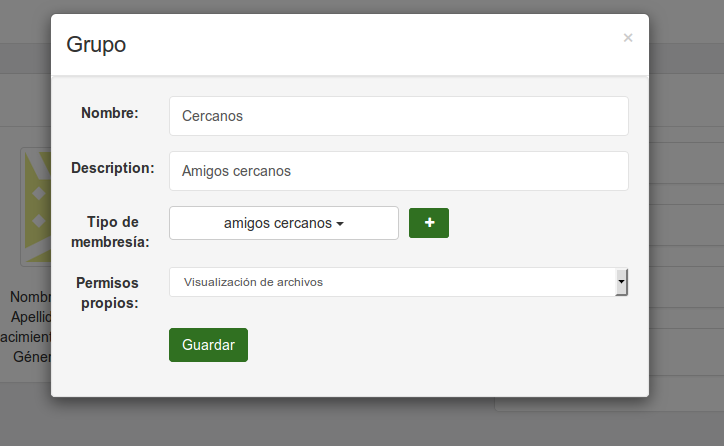
\includegraphics[width=0.5\textwidth]{img/nuevo_grupo}
	    	\caption{Formulario para la creación de nuevo grupo}
	    	\label{nuevo_grupo}
	    \end{figure}	    	    
	    
	    	    \begin{figure}[h]
	    	    	\centering
	    	    	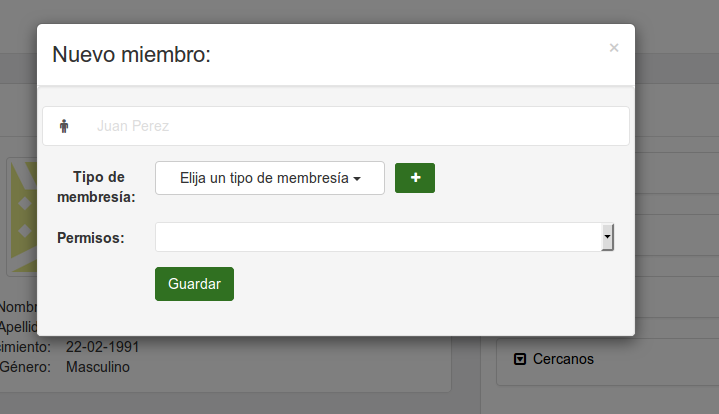
\includegraphics[width=0.5\textwidth]{img/nuevo_usuario_grupo}
	    	    	\caption{Formulario para añadir un usuario a un grupo}
	    	    	\label{nuevo_usuario_grupo}
	    	    \end{figure}	    	    
	    	    
	    	    	    \begin{figure}[h]
	    	    	    	\centering
	    	    	    	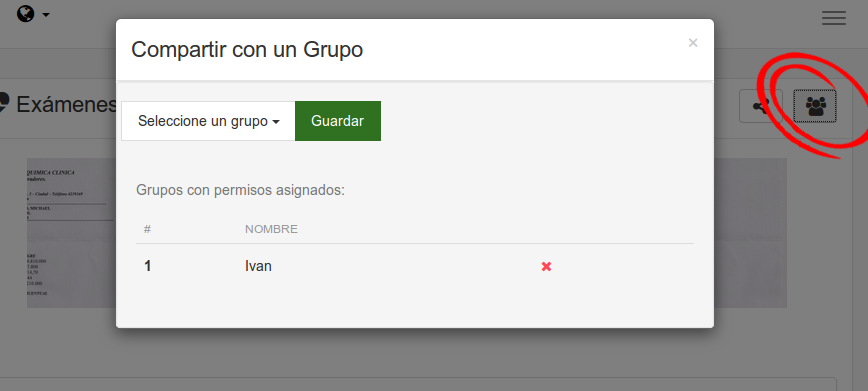
\includegraphics[width=0.5\textwidth]{img/compartir_analisis_grupo}
	    	    	    	\caption{Formulario para compartir un análisis con un grupo}
	    	    	    	\label{compartir_analisis_grupo}
	    	    	    \end{figure}	    	    
\clearpage	    	    	    	    
\subsection{Planificación y ejecución de Pruebas}
\subsubsection{Criterios de aceptación}

\begin{center}
\begin{longtable}{|p{0.5cm}|p{4cm}|p{4cm}|p{4.5cm}| }

	\hline 
		\rowcolor[gray]{0.9} 
		\multicolumn{4}{|c|}{\textbf{Criterio de aceptación}} \\
	\hline
    	\rowcolor[gray]{0.9} 
    	\multicolumn{1}{|c}{\textbf{Id}} & \multicolumn{1}{|c}{\textbf{Contexto}} &  \multicolumn{1}{|c}{\textbf{Evento}} & \multicolumn{1}{|c|}{\textbf{Resultado}} \\
    \hline
    	
1&Usuario autenticado, análisis existente, análisis pertenece al usuario, comentarios creados relacionados al análisis & Cuando el usuario autenticado solicita los comentarios del análisis & El sistema responderá con un código de estado 200 OK, devolverá una lista de comentarios del análisis ordenados por fecha y hora\\  \hline
% AnalysisAnalysisCommentList GET
 
2& Usuario autenticado, análisis existente, análisis pertenece al usuario autenticado, comentario pertenece a otro usuario   & Al intentar modificar el comentario & El sistema responderá con el código de estado 403 indicando la imposibilidad de actualización del comentario del análisis\\ \hline
% AnalysisCommentView PUT

3& Usuario autenticado, tipo de membresía de grupo existente, tipo de permiso existente & Cuando el usuario solicita crear un nuevo grupo & El sistema responderá con el código 200 CREATE, creará una instancia de Group y una nueva instancia de GroupMembership según el tipo de membresía de grupo, el tipo de permiso y perfil de usuario y la relaciona al grupo creado. Por último, devolverá los datos del grupo, id, name y description\\ \hline
% GroupList POST

4& Usuario autenticado, tipo de membresía no existe & Cuando el usuario solicite el tipo de membresía específico & El sistema responderá con el código de estado 404 NOT FOUND\\ \hline
% GroupMembershipTypeView GET

5& Usuario autenticado, tipo de medición existente, validaciones de unidad de medida existentes para el tipo de medida & cuando el usuario solicita por las validaciones & El sistema responde con el código de estado HTTP 200 FOUND y retorna la lista de validaciones de unidad de medición que restringen los valores del tipo de medición indicado\\ \hline
% TypeUnitValidationList GET



  \end{longtable}
\end{center}



\subsection{Retroalimentación de pruebas}
Aquí se realizará una conclusión general de lo que se descubrió en las pruebas.
        %
	\begin{itemize}
		\item \textbf{¿Qué fue bien?}
        	\begin{itemize}
				\item  Los comentarios registrados para el análisis de un usuario son visibles por el dueño del análisis
				\item Una ves comentado un análisis se crea correctamente la notificación y aparece entre las notificaciones pendientes de lectura para el usuario destino.
				\item Al crear un grupo se genera una membresía para el usuario según el tipo de membresía que haya establecido y, a su vez, queda como administrador del grupo. 
				\item Cuando un usuario es agregado a un grupo se crea la notificación correspondiente para el mismo.
				\item Al consultar por las validaciones de unidades de medida de un tipo de medida se obtiene correctamente una lista de validaciones con valores máximos y mínimos.
			\end{itemize}

   		\item \textbf{¿Qué se mejoró?}
        	\begin{itemize}
                \item \textbf{Cerrado} Se especifica, en el título de la notificación, el autor responsable de la misma.  El autor de una notificación es aquel que, mediante su acción en el sistema, genera la misma, destinada a otro usuario.
                \item \textbf{Cerrado} Obtención de thumbnail de archivos encriptados de análisis. Se añade soporte para archivos de análisis encriptados, al solicitar su thumbnail. Debido a que el archivo se encuentra encriptado en su ubicación de almacenamiento, el mismo se desencripta y se retorna en su forma original, no mediante un thumbnail del mismo.
                \item \textbf{Cerrado} Se añade el parámetro booleano opcional download (por defecto, False), que indica si el thumbnail debe visualizarse o enviarse como adjunto para ser descargado (True).
                \item \textbf{Cerrado} Implementación de recurso para obtener los análisis compartidos con el usuario. \textbf{MySharedAnalysesList}
                \begin{sloppypar}
                \item \textbf{Cerrado} Se añade a la clase Profile el atributo booleano is\_health\_professional, que indica si el perfil pertenece a un profesional médico.
                \end{sloppypar}
                \item \textbf{Cerrado} Se crea el recurso \textbf{MySharedAnalysisProfileList} que mediante el servicio GET, retorna todos los perfiles de usuario que son dueños de análisis sobre los cuales el usuario autenticado tiene permisos. 
                \item \textbf{Cerrado} Se permite la inclusión de caracteres numéricos en el campo symbol de MeasurementUnit. Esto es para poder cargar simbolos como m3, g/dm3, entre otros.
                \item \textbf{Cerrado} Se implementó el adaptador para la carga de archivos al sistema hosteado de almacenamiento ofrecido por google, Drive, para ello se relevo la api ofrecida por google y el uso del cliente para la comunicación entre YesDoc y el mismo. El siguiente diagrama [\ref{9-archivos-drive}] muestra el diseño actual para la gestión de archivos.   
			\end{itemize}
			
				\begin{figure}[h]
			        \centering
			        \includegraphics[width=0.9\textwidth]{img/dcd_archivos_drive}
			        \caption{Gestión de archivos con Drive.}
					\label{9-archivos-drive}
			    \end{figure}

   		\item \textbf{¿Qué se puede mejorar?}
        	\begin{itemize}
		        \item \textbf{Abierto} En el futuro se podrían implementar recursos que devuelvan resultados estadísticos de valor. Dada una gran cantidad de datos resulta muy útil sobre todo al usuario médico.
		        \item \textbf{Abierto} Se podría implementar medios por los cuáles diversos dispositivos puedan cargar automáticamente las medidas tomadas.
		        \item \textbf{Abierto} El usuario podría registrarse con cuentas de otros sistemas como puede ser facebook por ejemplo.
		        \item \textbf{Abierto} El almacenamiento de archivos y análisis podría hacerse de forma estructurada de acuerdo a las especialidades médicas que intervienen en la consulta o proceso de atención, diagnóstico y mejora.
		       
            \end{itemize}
        

	\end{itemize}
